%%%%%%%%%%%%%%%%%%%%%%%%%%%%%%%%%%%%%%%%%%%%%%%%%%%%%%%%%%%%%%%%%%%%%%%%%%%%%%%%%%
\begin{frame}[fragile]\frametitle{}
\begin{center}
{\Large Retrieval Augmented Generation (RAG)}
\end{center}
\end{frame}

% %%%%%%%%%%%%%%%%%%%%%%%%%%%%%%%%%%%%%%%%%%%%%%%%%%%%%%%%%%%
% \begin{frame}[fragile]\frametitle{Introduction}

% \begin{itemize}
% \item What is RAG? A new paradigm for generation tasks, combining retrieval and generation models.
% \item Motivation: Overcoming limitations of pure generative models in factual consistency, efficiency, and diversity.
% \item Impact: Improved performance in text summarization, question answering, and other NLP tasks.
% \end{itemize}	

% \end{frame}


%%%%%%%%%%%%%%%%%%%%%%%%%%%%%%%%%%%%%%%%%%%%%%%%%%%%%%%%%%%
\begin{frame}[fragile]\frametitle{Need for RAG}

\begin{itemize}
\item Industrial settings prioritize cost-conscious, privacy-respecting, and reliable solutions.
\item Prone to hallucinations, factual errors, and repetitive outputs.
\item Own/Private/Streaming/Latest data
\item Efficiency Concerns: Large generative models require extensive training data and high computational resources.
\item RAG vs Fine-tuning
% \item Companies, including startups, seek solutions with a return on investment rather than investing in talent or training models from scratch.
\item Recent research and chatbot releases demonstrate the capability to leverage knowledge beyond model weights.
% \item One approach is to iteratively call another neural network or language model (LM) to extract required information.
% \item Iteratively calling LM involves multiple interactions to extract information as shown in the provided image.g, as separating reasoning from factual information is not straightforward.
\end{itemize}	

\end{frame}


% %%%%%%%%%%%%%%%%%%%%%%%%%%%%%%%%%%%%%%%%%%%%%%%%%%%%%%%%%%%
% \begin{frame}[fragile]\frametitle{RAG in Iterations}


% \begin{center}
% 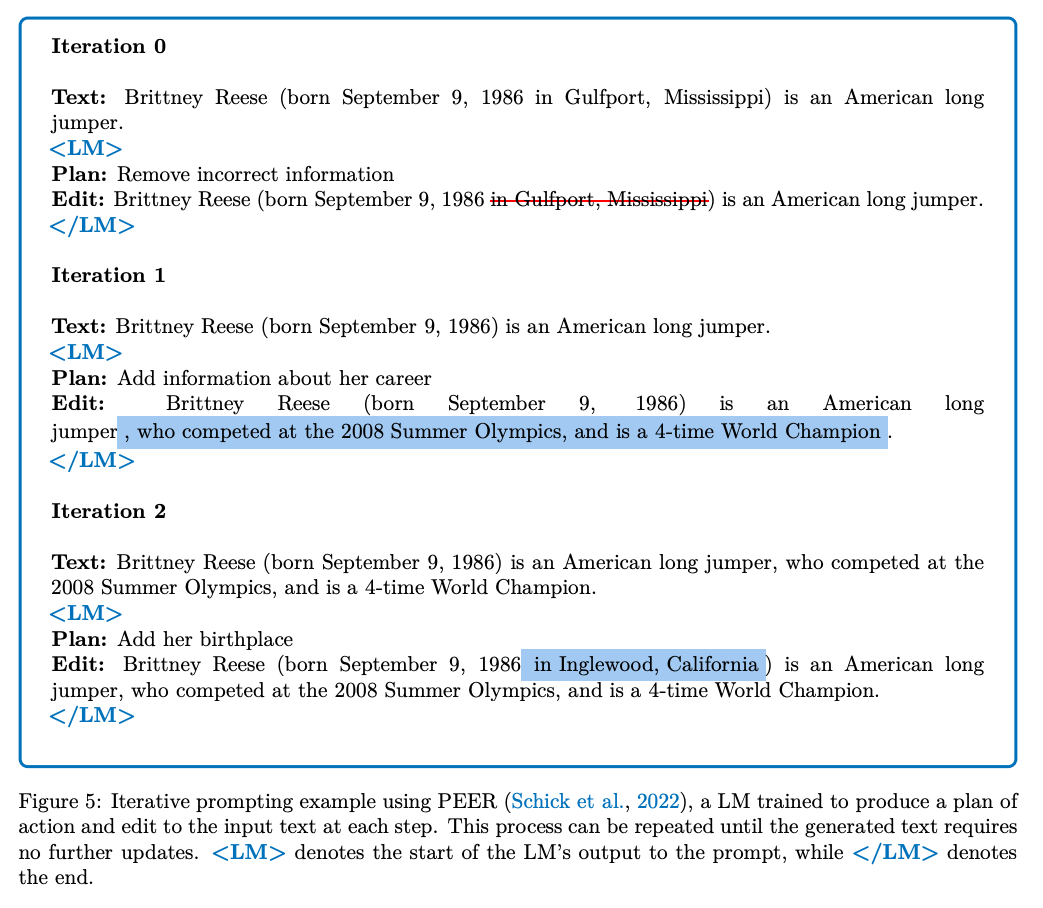
\includegraphics[width=0.8\linewidth,keepaspectratio]{chatgpt46}
% \end{center}

% {\tiny (Ref: Overview of Large Language Models - Aman AI)}

% \end{frame}

%%%%%%%%%%%%%%%%%%%%%%%%%%%%%%%%%%%%%%%%%%%%%%%%%%%%%%%%%%%
\begin{frame}[fragile]\frametitle{Retrieval Augmented Generation (RAG) for LLMs}
\begin{itemize}
  \item \textbf{Unlimited Knowledge:}
    \begin{itemize}
      \item RAG enables LLMs to access external sources, surpassing limitations of internal data.
      \item Allows exploration of proprietary documents and internet searches, broadening understanding.
      \item Introduces both Parametric and Non-Parametric Memory, enhancing models' knowledge.
      % \item Read the seminal paper on RAG - https://lnkd.in/gN2cAcXx.
    \end{itemize}
  
  \item \textbf{Easier to Update/Maintain:}
    \begin{itemize}
      \item Offers a cost-effective way to update and maintain %non-parametric memory in LLMs.
      \item Building a solid knowledge base minimizes ongoing maintenance financial burden.
      \item Pre-training expenses are mitigated, and fine-tuning is tailored to specific use cases.
      % \item Read Gopi's blog on cost implications of LLMs - https://lnkd.in/gJ-bT4RH.
    \end{itemize}
\end{itemize}

\end{frame}

%%%%%%%%%%%%%%%%%%%%%%%%%%%%%%%%%%%%%%%%%%%%%%%%%%%%%%%%%%%
\begin{frame}[fragile]\frametitle{Retrieval Augmented Generation (RAG) for LLMs (Contd.)}

\begin{itemize}
  \item \textbf{Confidence in Responses:}
    \begin{itemize}
      \item RAG enhances LLM confidence by providing extra context for more accurate responses.
      \item Practical boost to overall intelligence in generating responses.
    \end{itemize}
  
  \item \textbf{Context Awareness:}
    \begin{itemize}
      \item RAG makes LLMs adept at understanding context through added information.
      \item Results in responses that are not only accurate but also contextually fitting.
    \end{itemize}

  \item \textbf{Source Citation:}
    \begin{itemize}
      \item RAG provides access to sources, improving transparency in LLM responses.
      \item A step towards building trust in LLM systems.
      \item Explore text generation with citations in LLMs - Perplexity, Microsoft Co Pilot % https://lnkd.in/g2VEwRBK.
    \end{itemize}
\end{itemize}

\end{frame}

%%%%%%%%%%%%%%%%%%%%%%%%%%%%%%%%%%%%%%%%%%%%%%%%%%%%%%%%%%%
\begin{frame}[fragile]\frametitle{Retrieval Augmented Generation (RAG) for LLMs (Contd.)}

\begin{itemize}
  \item \textbf{Reduced Hallucinations:}
    \begin{itemize}
      \item RAG-enabled LLMs exhibit reduced creative misfires.
      \item Solid foundation of information keeps models focused and grounded.
      \item Pinecone explains more in this post - https://lnkd.in/gCfkDZYp.
    \end{itemize}

  \item \textbf{Practical Empowerment:}
    \begin{itemize}
      \item RAG shifts how we empower LLM systems practically.
      \item Focuses on expanding knowledge, building confidence, and maintaining grounded responses.
    \end{itemize}
\end{itemize}

\end{frame}



%%%%%%%%%%%%%%%%%%%%%%%%%%%%%%%%%%%%%%%%%%%%%%%%%%%%%%%%%%%
\begin{frame}[fragile]\frametitle{Important Questions}
\begin{itemize}
  \item Does the use case require external data access?
  \item Does the use case require changing foundation model style?
  \item Does the use case require addressing hallucinations?
  \item Is labeled training data available?
  \item Is citing the source of information important?
  \item How critical is system latency?
  \item What are the cost implications?
  \item What are the scalability requirements?
  \item Do we have the necessary expertise?
\end{itemize}
\end{frame}



%%%%%%%%%%%%%%%%%%%%%%%%%%%%%%%%%%%%%%%%%%%%%%%%%%%%%%%%%%%%%%%%%%%%%%%%%%%%%%%%%%
\begin{frame}[fragile]\frametitle{}
\begin{center}
{\Large Retrieval Augmented Generation (RAG) Workflow}
\end{center}
\end{frame}



%%%%%%%%%%%%%%%%%%%%%%%%%%%%%%%%%%%%%%%%%%%%%%%%%%%%%%%%%%%
\begin{frame}[fragile]\frametitle{RAG Architecture}


		\begin{center}
		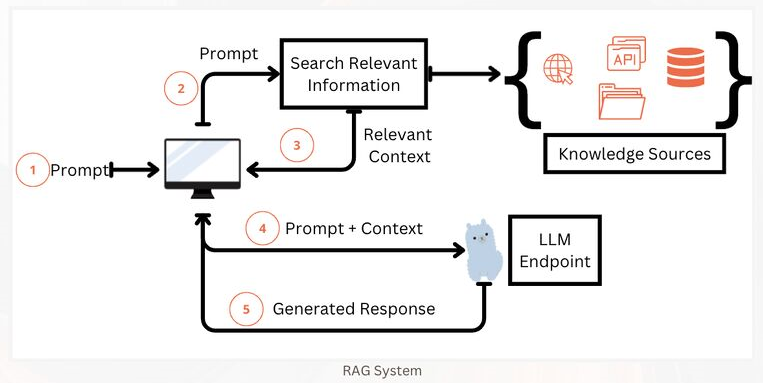
\includegraphics[width=\linewidth,keepaspectratio]{rag4a}
		\end{center}

{\tiny (Ref: RAG Architecture -Abhinav  Kimothi)}

\end{frame}

%%%%%%%%%%%%%%%%%%%%%%%%%%%%%%%%%%%%%%%%%%%%%%%%%%%%%%%%%%%
\begin{frame}[fragile]\frametitle{RAG Workflow}


		\begin{center}
		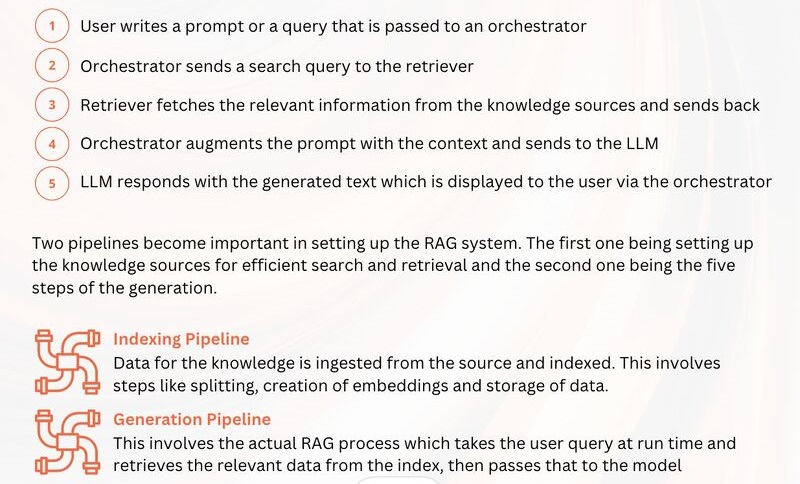
\includegraphics[width=\linewidth,keepaspectratio]{rag4b}
		\end{center}

{\tiny (Ref: RAG Architecture -Abhinav  Kimothi)}

\end{frame}

%%%%%%%%%%%%%%%%%%%%%%%%%%%%%%%%%%%%%%%%%%%%%%%%%%%%%%%%%%%
\begin{frame}[fragile]\frametitle{RAG in Steps}

The first step is to convert internal documents into a query-friendly format by embedding them using an embedding model.

\begin{itemize}
\item LLMs can gain external knowledge through information retrieval from memory units like external databases.
\item There are two types of information retrievers: dense and sparse.
\item Sparse retrievers use a sparse bag-of-words representation for documents and queries.
\item Dense (neural) retrievers utilize dense query and document vectors obtained from a neural network.
\item Retrieval-augmented LMs have shown strong performance in knowledge-intensive tasks, closing the performance gap compared to larger LMs with more parameters.
\item Save the text representing each embedding along with its corresponding pointer for future reference.
\end{itemize}

{\tiny (Ref: Overview of Large Language Models - Aman AI)}

\end{frame}

%%%%%%%%%%%%%%%%%%%%%%%%%%%%%%%%%%%%%%%%%%%%%%%%%%%%%%%%%%%
\begin{frame}[fragile]\frametitle{RAG in Steps}

Next we can start constructing the answer to a question/query of interest:

\begin{itemize}
\item Embed the question using the same Embedding Model as the knowledge base.
\item Use the resulting Vector Embedding to query the Vector Database and specify the desired number of retrieved vectors, representing the context for answering the query.
\item Perform an Approximate Nearest Neighbour (ANN) search in the Vector DB to find similar vectors in the Embedding/Latent space.
\item Map the returned Vector Embeddings to the corresponding text chunks.
\item Provide the question and retrieved context text chunks to the LLM via prompt, instructing it to use only the provided context for answering the question.
\item Ensure that prompt engineering is applied to ensure the LLM's answers are within expected boundaries, avoiding fabricated answers when there is no relevant data in the retrieved context.
\end{itemize}

{\tiny (Ref: Overview of Large Language Models - Aman AI)}

\end{frame}

%%%%%%%%%%%%%%%%%%%%%%%%%%%%%%%%%%%%%%%%%%%%%%%%%%%%%%%%%%%
\begin{frame}[fragile]\frametitle{RAG in Steps}

Next we can start constructing the answer to a question/query of interest:

\begin{itemize}
\item Use retrieval augmented generation (RAG) to enhance the knowledge base of an LM with relevant documents.
\item Employ vector databases like Pinecone, Chroma, Weaviate, Milvus, or LlamaIndex to augment LLMs.
\item RAG step-by-step process:
	\begin{itemize}
	\item Chunk, embed, and index documents in a vector database (VDB).
	\item Utilize (approximate) nearest neighbor techniques to match the query embedding of the claim advisor.
	\item Retrieve the relevant context from the VDB.
	\item Augment the LLM's prompt with the retrieved content.
	\end{itemize}

\item Consider LangChain or Google Vertex for prototyping or industrial applications, respectively.
\item Another approach is leveraging the search engine itself, as demonstrated by WebGPT, which can interact with a web browser, refine queries, navigate webpages, follow links, and cite sources.e within expected boundaries, avoiding fabricated answers when there is no relevant data in the retrieved context.
\end{itemize}

{\tiny (Ref: Overview of Large Language Models - Aman AI)}

\end{frame}

%%%%%%%%%%%%%%%%%%%%%%%%%%%%%%%%%%%%%%%%%%%%%%%%%%%%%%%%%%%
\begin{frame}[fragile]\frametitle{RAG in Steps}

Next we can start constructing the answer to a question/query of interest:

\begin{itemize}
\item Interact with the LLM through an API or direct interaction when working with prompts.
\item Configure parameters to customize prompt results:

\begin{itemize}
\item Temperature: Lower temperature values increase determinism, selecting the highest probable next token. Higher values introduce more randomness, encouraging diversity and creativity in outputs. Lower temperature can be suitable for fact-based QA, while higher temperature may benefit creative tasks like poem generation.
\item Top\_p: Using nucleus sampling, top\_p controls the determinism of the model's response generation. Lower values prioritize exact and factual answers, while higher values promote diverse responses.
\end{itemize}

\item It is generally recommended to modify only one parameter at a time.
\item Results may vary depending on the specific version of the LLM used.
\end{itemize}

{\tiny (Ref: Overview of Large Language Models - Aman AI)}

\end{frame}

%%%%%%%%%%%%%%%%%%%%%%%%%%%%%%%%%%%%%%%%%%%%%%%%%%%%%%%%%%%
\begin{frame}[fragile]\frametitle{Evaluation and Metrics}

\begin{itemize}
\item ROUGE for summarization
\item BLEU for generation
\item F1-score for question answering
\item Additional metrics for factual accuracy, diversity, and coherence
\end{itemize}	

\end{frame}

%%%%%%%%%%%%%%%%%%%%%%%%%%%%%%%%%%%%%%%%%%%%%%%%%%%%%%%%%%%
\begin{frame}[fragile]\frametitle{Pros and Cons of RAG}

\begin{itemize}
\item Pros: Improved factual accuracy, diversity, and efficiency compared to pure generation.
\item Cons: Increased complexity, potential bias introduced by the retrieval component, and dependency on external corpus quality.
\end{itemize}	

\end{frame}

%%%%%%%%%%%%%%%%%%%%%%%%%%%%%%%%%%%%%%%%%%%%%%%%%%%%%%%%%%%%%%%%%%%%%%%%%%%%%%%%%%
\begin{frame}[fragile]\frametitle{}
\begin{center}
{\Large Approaches in Details}
\end{center}
\end{frame}

%%%%%%%%%%%%%%%%%%%%%%%%%%%%%%%%%%%%%%%%%%%%%%%%%%%%%%%%%%%
\begin{frame}[fragile]\frametitle{Naive RAG Approach}

Simply retrieve texts and provide to language model as additional context during generation.

\begin{itemize}
\item Concept: Retrieve relevant documents from an external corpus before generation.
\item Steps: 1. Input query/topic. 2. Retrieve documents. 3. Generate summary/response based on retrieved documents.
\item Pros: Simple and effective for factual tasks.
\item Cons: May lack fluency and originality due to heavy reliance on retrieved text.
\end{itemize}	

\begin{center}
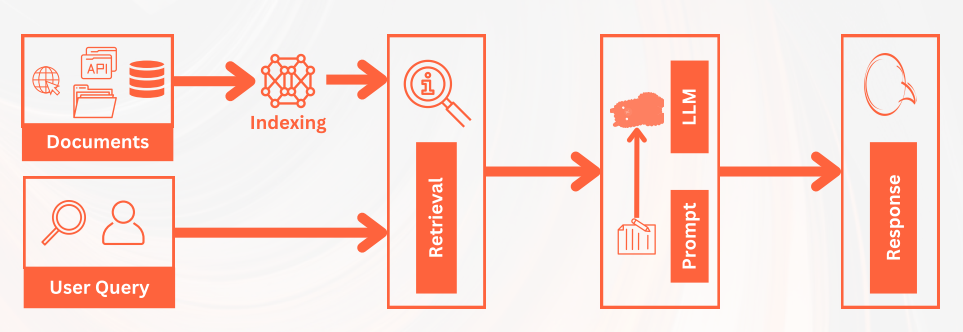
\includegraphics[width=0.8\linewidth,keepaspectratio]{rag1}

{\tiny (Ref: Progression of RAG Systems - Abhinav Kimothi )}
\end{center}		

\end{frame}

%%%%%%%%%%%%%%%%%%%%%%%%%%%%%%%%%%%%%%%%%%%%%%%%%%%%%%%%%%%
\begin{frame}[fragile]\frametitle{Challenges in Naive RAG}

\begin{itemize}
\item Retrieval Quality
	\begin{itemize}
	\item Low Precision leading to Hallucinations/Mid-air drops
	\item Low  Recall  resulting in  missing  relevant info
	\item Outdated information
	\end{itemize}
\item Augmentation
	\begin{itemize}
	\item Redundancy and Repetition when multiple retrieved documents have similar information
	\item Context Length challenges
	\end{itemize}
\item Generation Quality
	\begin{itemize}
	\item Generations are not grounded in the context 
	\item Potential of toxicity and bias in the response
	\item Excessive dependence on augmented context
	\end{itemize}
\end{itemize}	


{\tiny (Ref: Progression of RAG Systems - Abhinav Kimothi )}

\end{frame}

%%%%%%%%%%%%%%%%%%%%%%%%%%%%%%%%%%%%%%%%%%%%%%%%%%%%%%%%%%%
\begin{frame}[fragile]\frametitle{Advanced RAG Approaches}

To  address  the  inefficiencies  of  the  Naive  RAG  approach,  Advanced  RAG
approaches implement strategies focused on three processes:
\begin{itemize}
\item Pre-Retrieval
\item Retrieval
\item Post Retrieval
\end{itemize}	

More complex integration through various processing layers between retriever and generator modules.

\begin{itemize}
\item Hybrid Model: Jointly train retrieval and generation models for stronger synergy.
\item Conditional Attention: Dynamically weigh retrieved documents based on their relevance to the current generation stage.
\item Controllable Generation: Introduce mechanisms to steer generated content towards retrieved information.
\end{itemize}	

\end{frame}

%%%%%%%%%%%%%%%%%%%%%%%%%%%%%%%%%%%%%%%%%%%%%%%%%%%%%%%%%%%
\begin{frame}[fragile]\frametitle{Advanced RAG Approaches}

\begin{center}
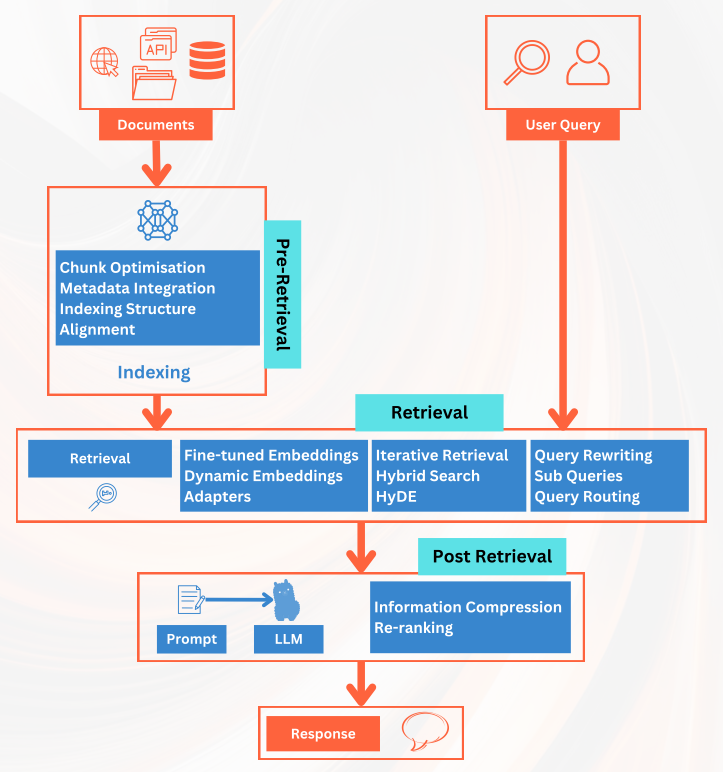
\includegraphics[width=0.55\linewidth,keepaspectratio]{rag2}

{\tiny (Ref: Progression of RAG Systems - Abhinav Kimothi )}
\end{center}	
\end{frame}


%%%%%%%%%%%%%%%%%%%%%%%%%%%%%%%%%%%%%%%%%%%%%%%%%%%%%%%%%%%
\begin{frame}[fragile]\frametitle{Advanced RAG Stages: Pre-retrieval}
\textbf{Chunk Optimization}

  \begin{itemize}
    \item Break external documents into appropriately sized chunks
    \item Decision factors: content type, user queries, and application needs
    \item No one-size-fits-all strategy; flexibility is crucial
    \item Current research explores techniques like sliding windows and "small2big" methods
  \end{itemize}
  
\textbf{Metadata Integration}

  \begin{itemize}
    \item Embed information like dates, purpose, chapter summaries, etc., into chunks
    \item Improves retriever efficiency by assessing similarity to metadata
  \end{itemize}
  

\end{frame}

%%%%%%%%%%%%%%%%%%%%%%%%%%%%%%%%%%%%%%%%%%%%%%%%%%%%%%%%%%%
\begin{frame}[fragile]\frametitle{Advanced RAG Stages: Pre-retrieval}
\textbf{Indexing Structure}
  \begin{itemize}
    \item Introduction of graph structures enhances retrieval
    \item Leverages nodes and their relationships
    \item Multi-index paths aimed at increasing efficiency
  \end{itemize}
  
\textbf{Alignment}
  \begin{itemize}
    \item Understanding complex data, like tables, can be tricky for RAG
    \item Improve indexing with counterfactual training
    \item Create hypothetical (what-if) questions to increase alignment
    \item Reduce disparity between documents
  \end{itemize}
\end{frame}

%%%%%%%%%%%%%%%%%%%%%%%%%%%%%%%%%%%%%%%%%%%%%%%%%%%%%%%%%%%
\begin{frame}[fragile]\frametitle{Advanced RAG Stages: Retrieval}
\textbf{Query Rewriting}
  \begin{itemize}
    \item Use rewriting approaches for better alignment between user queries and documents
    \item LLMs create pseudo-documents from the query for improved matching
    \item LLMs perform abstract reasoning; multi-querying for solving complex user queries
  \end{itemize}
\textbf{Hybrid Search Exploration}
  \begin{itemize}
    \item RAG system employs different types of searches: keyword, semantic, and vector
    \item Search type depends on user query and available data
  \end{itemize}
\end{frame}

%%%%%%%%%%%%%%%%%%%%%%%%%%%%%%%%%%%%%%%%%%%%%%%%%%%%%%%%%%%
\begin{frame}[fragile]\frametitle{Advanced RAG Stages: Retrieval}
\textbf{Sub Queries}
  \begin{itemize}
    \item Break down complex queries into sub-questions for each relevant data source
    \item Gather intermediate responses and synthesize a final response
  \end{itemize}
\textbf{Query Routing}
  \begin{itemize}
    \item Query router identifies downstream task and decides subsequent action for RAG system
    \item During retrieval, query router identifies most appropriate data source
  \end{itemize}
\textbf{Iterative Retrieval}
  \begin{itemize}
    \item Collect documents repeatedly based on query and generated response
    \item Create a more comprehensive knowledge base
  \end{itemize}
\end{frame}

%%%%%%%%%%%%%%%%%%%%%%%%%%%%%%%%%%%%%%%%%%%%%%%%%%%%%%%%%%%
\begin{frame}[fragile]\frametitle{Advanced RAG Stages: Retrieval}
\textbf{Recursive Retrieval}
  \begin{itemize}
    \item Iteratively retrieves documents and refines search queries based on previous results
    \item Continuous learning process
  \end{itemize}
\textbf{Adaptive Retrieval}
  \begin{itemize}
    \item Enhance RAG framework by empowering LLMs to proactively identify suitable moments and content for retrieval
    \item Improve efficiency and relevance of information obtained
    \item Dynamically choose when and what to retrieve for more precise and effective results
  \end{itemize}
\end{frame}

%%%%%%%%%%%%%%%%%%%%%%%%%%%%%%%%%%%%%%%%%%%%%%%%%%%%%%%%%%%
\begin{frame}[fragile]\frametitle{Advanced RAG Stages: Retrieval}
\textbf{Hypothetical Document Embeddings (HyDE)}
  \begin{itemize}
    \item LLM-based HyDE forms a hypothetical document in response to a query
    \item Embeds it and retrieves real documents similar to this hypothetical one
    \item Emphasizes similarity between embeddings of different answers
  \end{itemize}
\textbf{Fine-tuned Embeddings}
  \begin{itemize}
    \item Tailor embedding models to improve retrieval accuracy
    \item Particularly useful in specialized domains dealing with uncommon or evolving terms
    \item Fine-tuning utilizes training data generated with language models grounded in document chunks
  \end{itemize}
\end{frame}


%%%%%%%%%%%%%%%%%%%%%%%%%%%%%%%%%%%%%%%%%%%%%%%%%%%%%%%%%%%
\begin{frame}[fragile]\frametitle{Advanced RAG Stages: Post-retrieval}
\textbf{Information Compression}
  \begin{itemize}
    \item Retriever proficient in extracting relevant information from extensive knowledge bases
    \item Challenge: Managing vast amount of information within retrieval documents
    \item Compress retrieved information to extract the most relevant points
    \item Information passed to LLM after compression
  \end{itemize}
\textbf{Reranking}
  \begin{itemize}
    \item Re-ranking model crucial for optimizing the document set retrieved by the retriever
    \item Rearrange document records to prioritize the most relevant ones at the top
    \item Manages the total number of documents effectively
    \item Resolves challenges related to context window expansion during retrieval
    \item Improves efficiency and responsiveness
  \end{itemize}
\end{frame}


% %%%%%%%%%%%%%%%%%%%%%%%%%%%%%%%%%%%%%%%%%%%%%%%%%%%%%%%%%%%
% \begin{frame}[fragile]\frametitle{Modular RAG Architectures}

% Separate retriever and generator modules that can be independently improved.

% \begin{itemize}
% \item Decomposed Modules: Separate modules for retrieval, filtering, and generation, allowing for customization.
% \item Allows components like search, memory, and reranking modules to be configured
% \item Fine-tuning Flexibility: Adapting individual modules to specific tasks or data domains.
% \item Interpretability Advantages: Easier to analyze the contribution of each module to the final output.
% \end{itemize}	

% \end{frame}



% %%%%%%%%%%%%%%%%%%%%%%%%%%%%%%%%%%%%%%%%%%%%%%%%%%%%%%%%%%%
% \begin{frame}[fragile]\frametitle{Modular RAG Architectures}

% \begin{center}
% 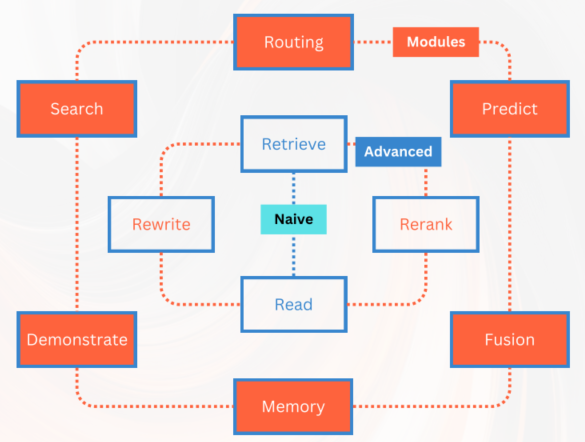
\includegraphics[width=0.8\linewidth,keepaspectratio]{rag3}

% {\tiny (Ref: Progression of RAG Systems - Abhinav Kimothi )}
% \end{center}

% \end{frame}

% %%%%%%%%%%%%%%%%%%%%%%%%%%%%%%%%%%%%%%%%%%%%%%%%%%%%%%%%%%%
% \begin{frame}[fragile]\frametitle{Some RAG Modules}

  % \begin{itemize}
    % \item \textbf{Search:}
          % \begin{itemize}
              % \item Perform search on different data sources
              % \item Customized for various data sources
              % \item Increase source data for better response generation
          % \end{itemize}
    % \item \textbf{Memory:}
          % \begin{itemize}
              % \item Leverage parametric memory capabilities of the Language Model (LLM)
              % \item Guide retrieval using retrieval-enhanced generator
              % \item Create an unbounded memory pool iteratively
          % \end{itemize}
    % \item \textbf{Fusion (RAG-Fusion):}
          % \begin{itemize}
              % \item Overcome limitations of traditional search systems
              % \item Multi-query approach, expanding user queries into diverse perspectives
              % \item Conduct parallel vector searches for original and expanded queries
              % \item Intelligently re-rank and optimize results
          % \end{itemize}
    % \item \textbf{Extra Generation:}
          % \begin{itemize}
              % \item Generate context using Language Model (LLM)
              % \item Address issues of repetition and irrelevant details in retrieved content
          % \end{itemize}
    % \item \textbf{Task Adaptable Module:}
          % \begin{itemize}
              % \item Make RAG adaptable to various downstream tasks
              % \item Develop task-specific end-to-end retrievers with minimal examples
              % \item Demonstrate flexibility in handling different tasks
          % \end{itemize}
  % \end{itemize}

% \end{frame}

% %%%%%%%%%%%%%%%%%%%%%%%%%%%%%%%%%%%%%%%%%%%%%%%%%%%%%%%%%%%
% \begin{frame}[fragile]\frametitle{Further RAG Variants and Advancements}

% \begin{itemize}
% \item Dense Passage Retrieval
% \item Transformer-based RAG models
% \item Multi-stage RAG with diverse retrieval strategies
% \item Explainable RAG for interpretability
% \item RAG for low-resource languages
% \end{itemize}	

% \end{frame}


%%%%%%%%%%%%%%%%%%%%%%%%%%%%%%%%%%%%%%%%%%%%%%%%%%%%%%%%%%%%%%%%%%%%%%%%%%%%%%%%%%
\begin{frame}[fragile]\frametitle{}
\begin{center}
{\Large RAG vs SFT (Supervised Fine - Tuning)}
\end{center}
\end{frame}




%%%%%%%%%%%%%%%%%%%%%%%%%%%%%%%%%%%%%%%%%%%%%%%%%%%%%%%%%%%
\begin{frame}[fragile]\frametitle{RAG \& SFT: Complementary Techniques}
% \begin{itemize}
  % \item RAG \& SFT are complementary, not competing methods.
  % \item RAG enhances non-parametric memory without changing parameters.
  % \item SFT changes parameters, impacting parametric memory.
% \end{itemize}
\textbf{RAG Features}
\begin{itemize}
  \item Connects to dynamic external data sources.
  \item Reduces hallucinations.
  \item Increases transparency in source of information.
  \item Works well with very large foundation models.
  \item Does not impact style, tone, vocabulary.
\end{itemize}
\textbf{SFT Features}
\begin{itemize}
  \item Changes style, vocabulary, tone of foundation model.
  \item Can reduce model size.
  \item Useful for deep domain expertise.
  \item May not address hallucinations.
  \item No improvement in transparency (black box models).
\end{itemize}
\end{frame}

%%%%%%%%%%%%%%%%%%%%%%%%%%%%%%%%%%%%%%%%%%%%%%%%%%%%%%%%%%%
\begin{frame}[fragile]\frametitle{Use Case Considerations for RAG \& SFT}
Use both if parametric and non-parametric memory changes are needed.

\begin{itemize}
  \item Access to dynamic external data source.
  \item Resolving hallucinations.
  \item Transparency in source of information.
  \item SFT requires access to labeled training data.
\end{itemize}
\end{frame}

%%%%%%%%%%%%%%%%%%%%%%%%%%%%%%%%%%%%%%%%%%%%%%%%%%%%%%%%%%%
\begin{frame}[fragile]\frametitle{Important Use Case Considerations}


		\begin{center}
		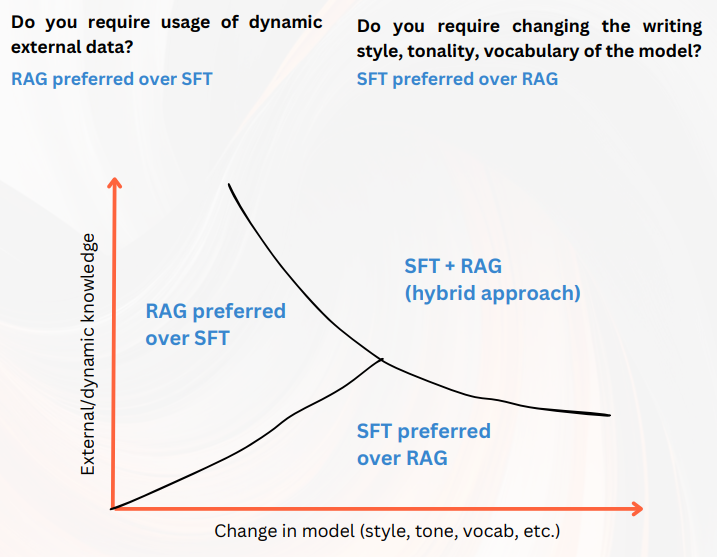
\includegraphics[width=0.8\linewidth,keepaspectratio]{rag24}
		\end{center}

{\tiny (Ref: Generative AI with Large Language Model - Abhinav  Kimothi)}

\end{frame}

%%%%%%%%%%%%%%%%%%%%%%%%%%%%%%%%%%%%%%%%%%%%%%%%%%%%%%%%%%%
\begin{frame}[fragile]\frametitle{Other Considerations}
\begin{itemize}
  \item \textbf{Latency:} RAG introduces inherent latency due to search and retrieval.
  \item \textbf{Scalability:} RAG pipelines are modular and scalable; SFT requires retraining.
  \item \textbf{Cost:} Both methods require upfront investment; costs vary.
  \item \textbf{Expertise:} RAG pipelines are moderately simple with frameworks; SFT needs deep understanding and training data creation.
\end{itemize}
\end{frame}

%%%%%%%%%%%%%%%%%%%%%%%%%%%%%%%%%%%%%%%%%%%%%%%%%%%%%%%%%%%%%%%%%%%%%%%%%%%%%%%%%%
\begin{frame}[fragile]\frametitle{}
\begin{center}
{\Large Limitations}
\end{center}
\end{frame}

%%%%%%%%%%%%%%%%%%%%%%%%%%%%%%%%%%%%%%%%%%%%%%%%%%%%%%%%%%%
\begin{frame}[fragile]\frametitle{Failure Points of RAG Systems}


		\begin{center}
		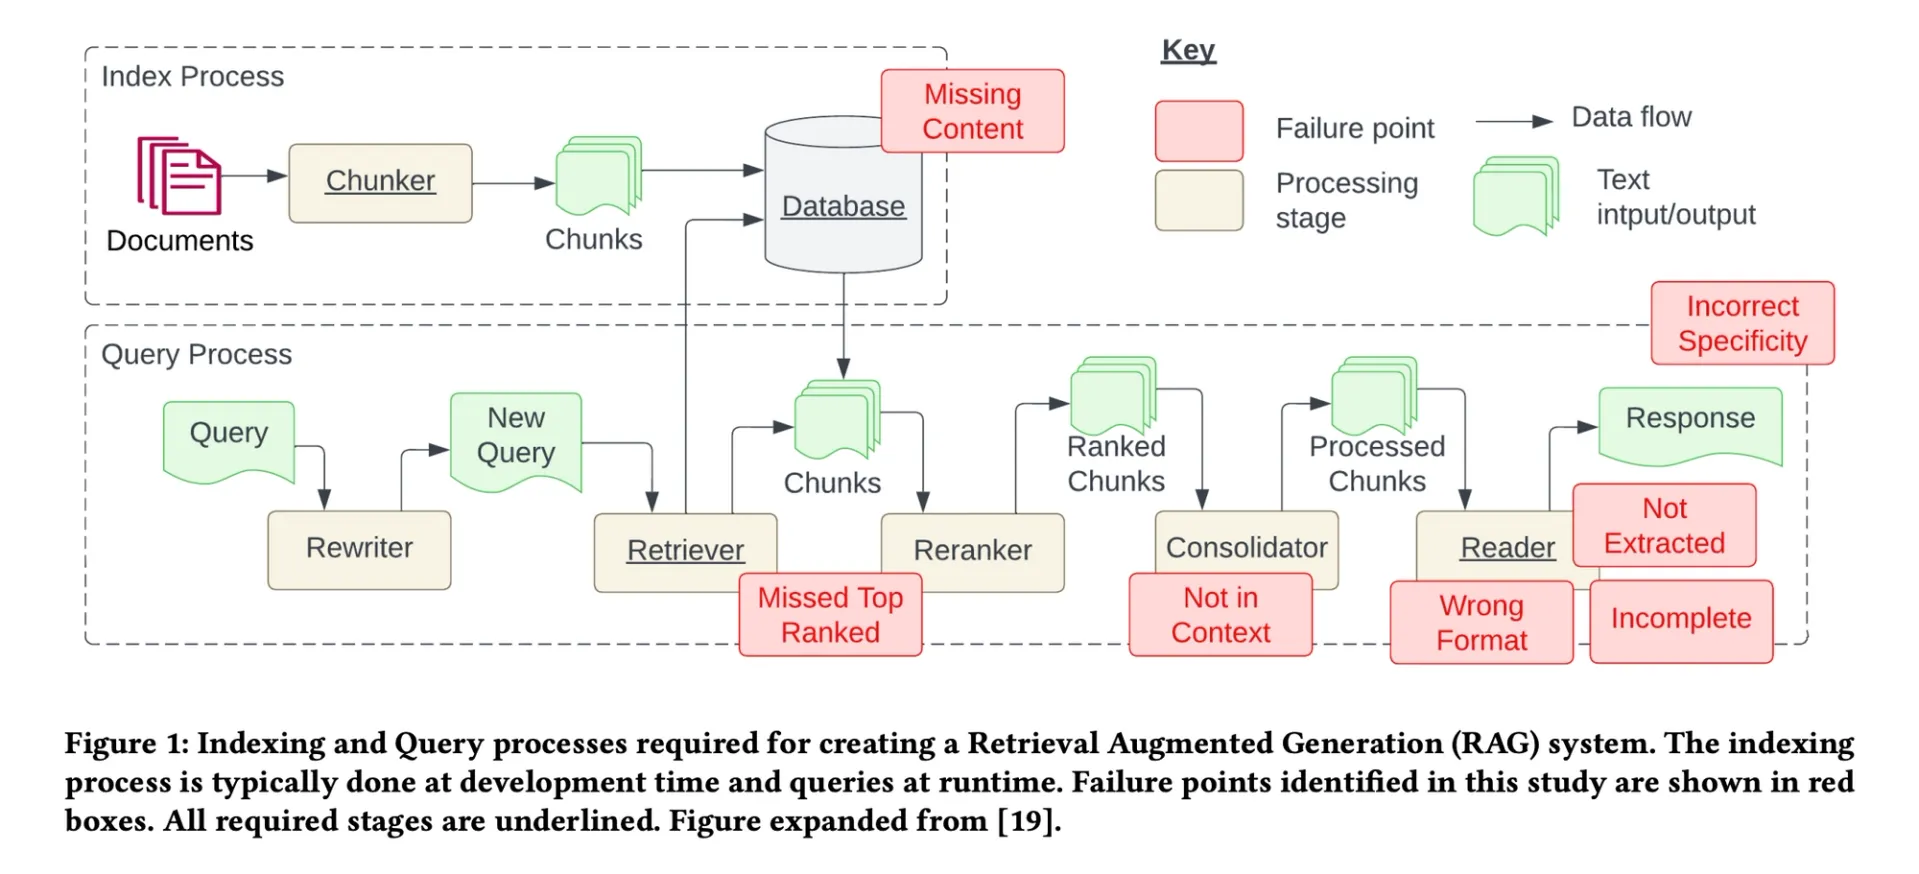
\includegraphics[width=0.8\linewidth,keepaspectratio]{rag34}
		\end{center}

{\tiny (Ref: Mastering RAG: How To Architect An Enterprise RAG System - Pratik Bhavsar)}

\end{frame}

%%%%%%%%%%%%%%%%%%%%%%%%%%%%%%%%%%%%%%%%%%%%%%%%%%%%%%%%%%%
\begin{frame}[fragile]\frametitle{Failure Points}
\begin{itemize}
  \item \textbf{Missing Content (FP1):}
    \begin{itemize}
        \item Question without answer in available documents.
        \item Ideal response: "Sorry, I don’t know."
        \item Risk of system being misled for questions without clear answers.
    \end{itemize}
  
  \item \textbf{Missed Top Ranked Documents (FP2):}
    \begin{itemize}
        \item Answer in document, but not ranked high enough.
        \item Only top K documents returned (K based on performance).
        \item Theoretical ranking vs. practical limitations.
    \end{itemize}
  
  \item \textbf{Not in Context - Consolidation Strategy Limitations (FP3):}
    \begin{itemize}
        \item Relevant answer retrieval hindered during consolidation.
        \item Occurs with a substantial number of returned documents.
        \item Challenge in incorporating retrieved documents into context.
    \end{itemize}
  
  \item \textbf{Not Extracted (FP4):}
    \begin{itemize}
        \item Answer present, but model fails to extract correct information.
        \item Occurs with excessive noise or conflicting information.
    \end{itemize}
  
  \item \textbf{Wrong Format (FP5):}
    \begin{itemize}
        \item Question involves specific format (table/list), but model disregards.
        \item Failure to follow instruction for information extraction.
    \end{itemize}
  
  \item \textbf{Incorrect Specificity (FP6):}
    \begin{itemize}
        \item Response lacks required specificity or is overly specific.
        \item Predetermined outcomes may lead to incorrect specificity.
        \item Unclear user questions may result in overly general responses.
    \end{itemize}
  
  \item \textbf{Incomplete (FP7):}
    \begin{itemize}
        \item Accurate answers lacking some information present in context.
        \item Example: Key points covered in multiple documents.
        \item Approach of asking separate questions for better results.
    \end{itemize}
\end{itemize}

{\tiny (Ref: Mastering RAG: How To Architect An Enterprise RAG System - Pratik Bhavsar)}

\end{frame}

%%%%%%%%%%%%%%%%%%%%%%%%%%%%%%%%%%%%%%%%%%%%%%%%%%%%%%%%%%%%%%%%%%%%%%%%%%%%%%%%%%
\begin{frame}[fragile]\frametitle{}
\begin{center}
{\Large Applications}
\end{center}
\end{frame}


%%%%%%%%%%%%%%%%%%%%%%%%%%%%%%%%%%%%%%%%%%%%%%%%%%%%%%%%%%%
\begin{frame}[fragile]\frametitle{Applications and Use Cases}

\begin{itemize}
\item Code generation in software development
\item Creative writing and storytelling
\item Educational material generation
\item Personalized product descriptions
\item many many more \ldots
\end{itemize}	

\end{frame}


%%%%%%%%%%%%%%%%%%%%%%%%%%%%%%%%%%%%%%%%%%%%%%%%%%%%%%%%%%%
\begin{frame}[fragile]\frametitle{Open Source Resources and Tools}

\begin{itemize}
\item LangChain, LlamaIndex like frameworks
\item Transformers library, Hugging Face model hub
\item Datasets and evaluation benchmarks
\end{itemize}	

\end{frame}



%%%%%%%%%%%%%%%%%%%%%%%%%%%%%%%%%%%%%%%%%%%%%%%%%%%%%%%%%%%
\begin{frame}[fragile]\frametitle{LangChain Implementation}

\begin{itemize}
\item Open-source framework: Designed specifically for modular RAG architectures.
\item Modular Components: Retrieval models, document ranking algorithms, and various generation models.
\item Customizable Pipelines: Define the flow of information between modules for specific tasks.
\end{itemize}	

\end{frame}

%%%%%%%%%%%%%%%%%%%%%%%%%%%%%%%%%%%%%%%%%%%%%%%%%%%%%%%%%%%
\begin{frame}[fragile]\frametitle{LangChain Case Studies}

\begin{itemize}
\item Text Summarization: Achieves state-of-the-art performance on benchmarks like CNN/Daily Mail and ROUGE.
\item Question Answering: Improves factual accuracy and answerability compared to pure generative models.
\item Other Applications: News writing, dialogue generation, and abstractive text editing.
\end{itemize}	

\end{frame}
